\documentclass[10pt,twocolumn,letterpaper]{article}
\usepackage{graphicx}
\usepackage{amsmath}
\usepackage{amssymb}
\usepackage{booktabs}
\usepackage{nicefrac}
\usepackage{algorithm}
\usepackage[algo2e]{algorithm2e} 
\usepackage{multirow}
\usepackage[pagebackref,breaklinks,colorlinks]{hyperref}

% Support for easy cross-referencing
\usepackage[capitalize]{cleveref}
\crefname{section}{Sec.}{Secs.}
\Crefname{section}{Section}{Sections}
\Crefname{table}{Table}{Tables}
\crefname{table}{Tab.}{Tabs.}

\begin{document}
\nocite{*}

\begin{figure}
    \centering
        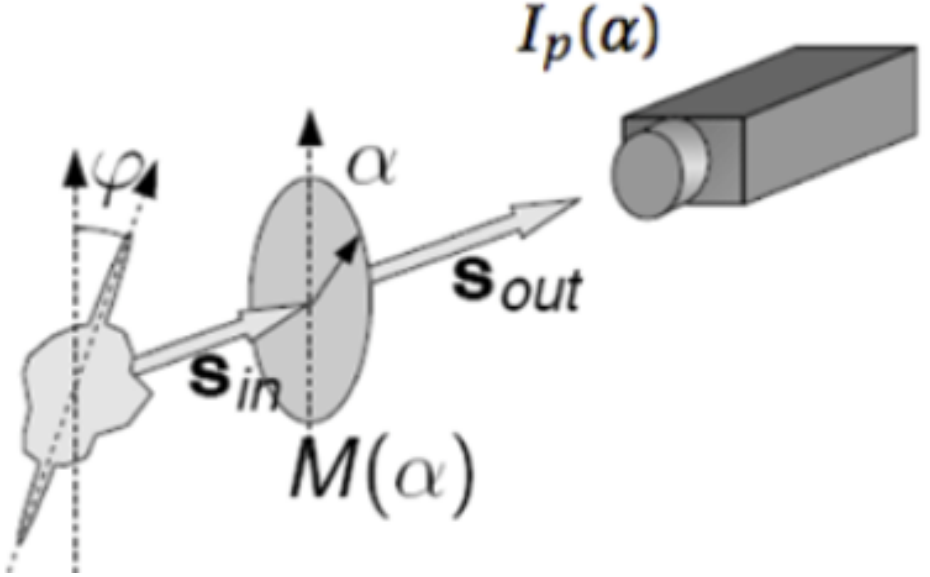
\includegraphics[width=7cm,height=4cm]{Exam/images/Fig_1.png} 
    \caption{The polarization device principle.}
    \label{fig:fig_1}
\end{figure}


of the light is that after being reflected, an unpolarized light
wave become partially linearly polarized depending on the
surface normal and on the refractive index of the material it
impinges on \cite{_8_}, [9], [15]. The reflected partially linearly
polarized light is described by a measurable vector, named
the Stokes vector $S = [S_{0},S_{1},S_{2}]$.  The first component $S_{0}$ relates to the object intensity, the two others describe the
physical properties of the object. From these three components, other physical properties are derived such as the light
magnitude \textit{I}, the degree of polarization (DOP) $\rho$and the
angle of polarization (AOP) $\varphi$ [16]. In order to measure the
polarization parameters, at least three images are required.
For this purpose, a rotating linear polarizer around three angles $(\alpha_{i})_{i=1:3}$ is placed in front of the camera. Figure.\labelcref{fig:fig_1} gives
an example of a polarization device. For each angle $(\alpha_{i})$  an
intensity \textit{I} $(\alpha_{i})$is measured by the camera. The relationship
between the acquired images and the Stokes vectors is given
by :

\begin{equation}
    \textit{I}(\alpha_{i}) = \frac{1}{2}[1,cos(2\alpha_{i}),sin(2\alpha_{i})].[S_{0},S_{1},S_{2}]^t
\end{equation}

The DOP is calculated as $\rho = \frac{\sqrt{S_{1}^2+S_{2}^2}}{S_{0}}$ and the AOP as $\varphi = \frac{1}{2}tan^{-1}\frac{S_{2}}{S_{1}}$


\section{FEATURE EXTRACTION}
\subsection{Polarisation feature selection}

\begin{figure}
    \centering
    \begin{tabular}{c c} % mettre des choses dans un tableau
        Original image & Angle of Polarization \\
        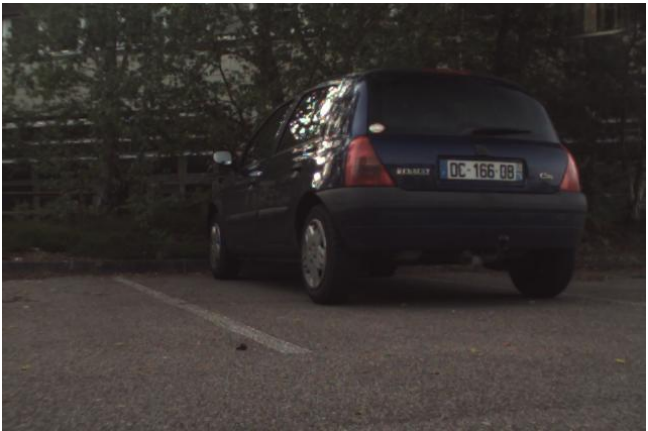
\includegraphics[width=5cm,height=3cm]{Exam/images/Fig_2_1.png} &
        \title{Angle of Polarization}
        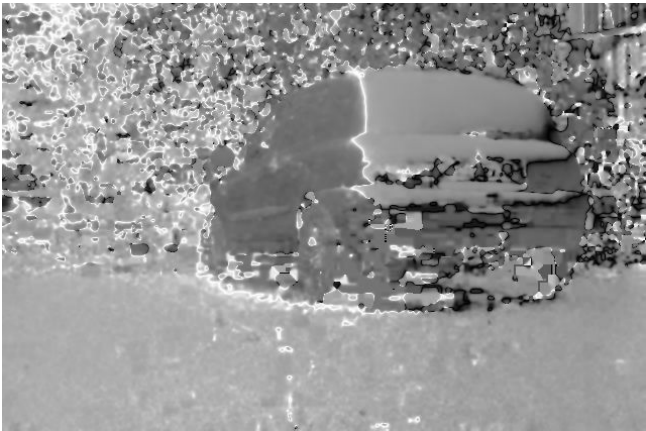
\includegraphics[width=5cm,height=3cm]{Exam/images/Fig_2_2.png} 
    \end{tabular}
    \caption{The original image and its corresponding AOP.}
    \label{fig:fig2}
\end{figure}

Because of the noisy nature of the polarization parameters,
a feature selection is required to find the most informative
polar-based feature for the detection model training. In our
case, the feature selection procedure is trained by the Dalal-Trigg detector \cite{_1_} by replacing the HOG feature by the polarization features.
To train the Dalal-Trigg detector, similar to the original
HOG features, the polarization features are extracted based
on blocks and cells. A 8⇥8 block was divided into four 4⇥4
cells. For each pixel in the cell, a feature vector is extracted,
which contains the 3-dimensional Stokes vector, the DOP ($\rho$) Because of the noisy nature of the polarization parameters,
a feature selection is required to find the most informative
polar-based feature for the detection model training. In our
case, the feature selection procedure is trained by the Dalal-Trigg detector [1] by replacing the HOG feature by the polarization features.
To train the Dalal-Trigg detector, similar to the original
HOG features, the polarization features are extracted based
on blocks and cells. A 8⇥8 block was divided into four 4⇥4
cells. For each pixel in the cell, a feature vector is extracted,
which contains the 3-dimensional Stokes vector, the DOP ($\varphi$). The feature vector $[S_{0},S_{1},S_{2},\rho,\varphi]$ of a cell is represented by the mean feature vector of all the pixels inside the cell. Each cell holds a 5-dimensional feature
vector. The feature vector of the block is the concatenation
of the feature vectors from the four cells. The derived 20 dimational features $\phi_{20-d}$ of all the examples are used to
train the Dalal-trigg detector in order to get the filter $f$ that
indicates the weight of each feature. Larger weight is, better
the relevancy of the corresponding feature. The advantage of
the feature selection is twofold : first, it allows to leverage
from the most relevant polarimetric information and second,
it reduces the dimension of the feature vector, making the detection faster.

By applying the feature selection process presented
above, the AOP was selected as the most informative feature with regards to the car detection purpose.

\subsection{The Angle of polarization}

The AOP refers to the direction of the polarization of the reflected light. It is determined by the angle of the incident
light (generally for outdoor applications, the incident light is
assumed to be unpolarized), the surface orientation of the object and the material of the object. For rough surface, as surface orientations of neighboring pixels change a lot, the AOP
changes in an irregularly way. For smooth surfaces, however,
the AOP changes smoothly and continuously. Up to the road
scenes analysis, especially for car detection tasks, the AOP on
the car surfaces changes gradually according to the surface
geometry structure, while it is noisy for other objects. This
phenomena is illustrated in Figure. \labelcref{fig:fig2} where the AOP image
on the tree area is highly noisy, on the road it is better but still
much noisy than on the car. It can be observed that the AOP
image describes the geometry structure of the car, which is
even more clear than that from the color image.

where the AOP image
on the tree area is highly noisy, on the road it is better but still
much noisy than on the car. It can be observed that the AOP
image describes the geometry structure of the car, which is
even more clear than that from the color image.

\section{DETECTION MODEL}

\begin{figure}
    \centering
        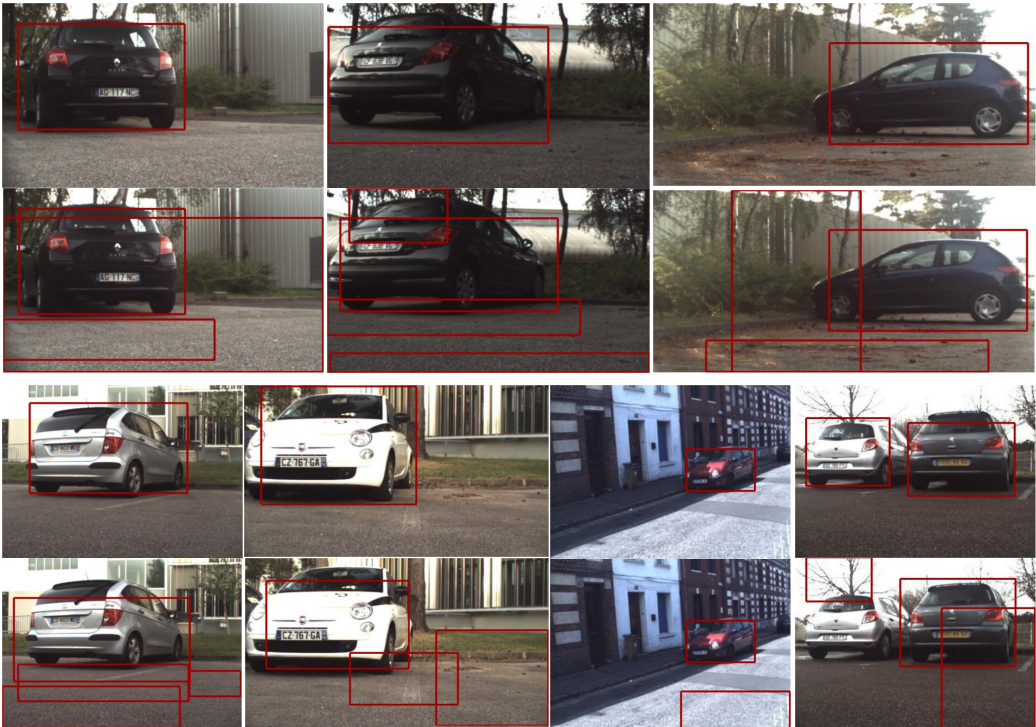
\includegraphics[width=7cm,height=4cm]{Exam/images/Fig_5.png} 
    \caption{ Detection results. The first and third rows refer to the
                polar-based model whereas the second and fourth rows are the
                corresponding color-only based model.}
    \label{fig:fig_5}
\end{figure}

\begin{table}[]
    \centering
    \begin{tabular}{|c|c|c|c|c|c|}
        \hline
        Source & AOP & 20 - $d$ & 20 - $d$ + color & color & AOP +color\\
        \hline
        AP($\%$) & 31.8 & 53.8 & 62.8 & 62.7 & \bold{66.1} \\
        \hline
    \end{tabular}
    \caption{The Average Precision (AP) rate}
    \label{tab:tab_1}
\end{table}

The DPM model proposed by Felzenswalb \cite{_2_} is known to be
an efficient method that handles the intraclass variations of an
object. The DPM is a filter-based detector applied throughout does not provide comparable results, this is because the noise
still strongly present in polarization acquisitions.

This result confirms that once the AOP is properly fused
with the color model, it provides complementary information
that improves the AP by $3.4\%$. The 20 - $d$ is more stable
than the AOP, however, with all the redundant features and the
more complex model, it almost does not improve the colorbased result
($0.1\%$ cancan be even neglected). Moreover, the
AOP alone achieves $31.8\%$ of AP, which is important comparing to the
$53.8\%$ performed by the whole polarization feature 20 - $d$. This result shows that the AOP has an important impact on the detection process. According to the above
analysis, it can be concluded that our proposed pre-selection
method is valid. By using the selected feature (AOP) and the
proposed fusion rule, the polarization features provided useful
information which improved and reinforced the color-based
method.

To evaluate the improvement provided by the fusion of
AOP $+ color$,we compare the detected bounding box by
AOP $+ color$ method with the color-only one. This comparison is shown in Figure. \labelcref{fig:fig5},The first and third rows show the
results of the detection with the AOP $+ color$ fusion and the
second and fourth rows show the corresponding color-only
detection method. It is worth to note that, after fusing the
two different sources of information via the proposed fusion
scheme, while keeping the true positive bounding boxes, the
false detection are effectively removed.


\begin{figure}
    \centering
        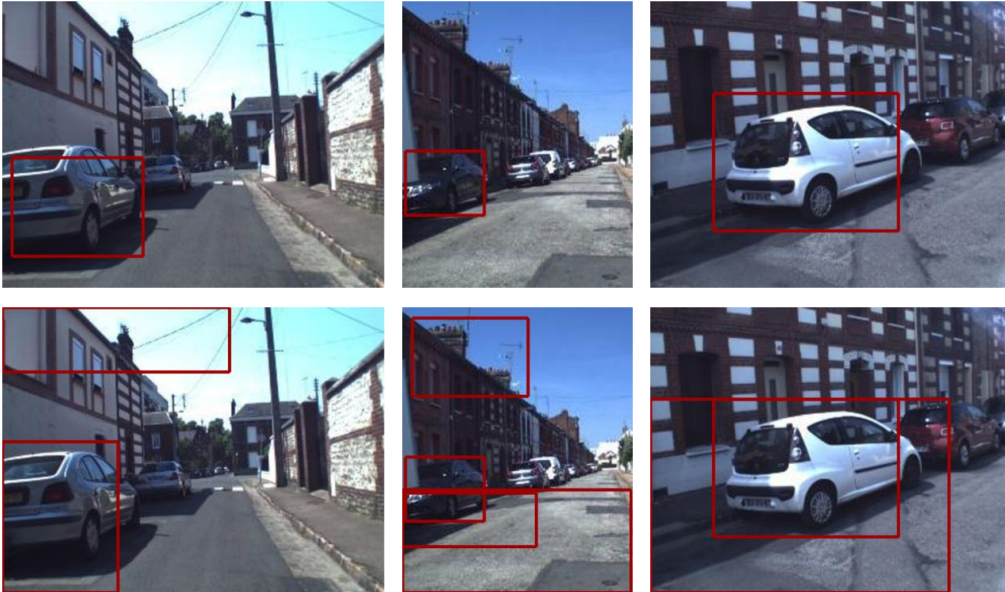
\includegraphics[width=7cm,height=4cm]{Exam/images/Fig_6.png} 
    \caption{ Main limitations. False alarms are reduced however
            not new true positive detection boxes are generated.}
    \label{fig:fig_6}
\end{figure}

\section{DISCUSSION}

The detection results have shown that the proposed methodology
largely reduced the false detection rate and enhance
the robustness of the model. Our approach confirmed that
polarization-based features can provide useful information for
car detection. False alarms were reduced by a simple but effective
fusion rule. However, as it can be seen in Figure. \labelcref{fig:fig_6},
the polarization-based feature model does not generate new
true positive detection boxes. This limitation is caused by the
And-fusion used scheme, which is too much selective.

Our first objective by this work is to prove that polarization is the
suitable alternative to color-based models for improving the detection 
result. This first observation is encouraging to continue our 
investigation in this direction. As a future work, the polarization
feature should be properly fused
with the color one inside a training loop. A stable model
which integrates the color-based feature and the polar-based
feature by an early-based fusion scheme might be able to
both reduce the false detection and produce new true positive bounding
boxes as well. Other more recent methods like
the transfer learning based on the Deep learning networks,
that shown interesting performances in several computer vision 
applications even for vehicle detection [20], should be
tested in the polarization domain.

The enhancing of the polarization images quality is not to
be missed. Because of the noise reaching polarization aquisitions, it
was difficult to leverage from the whole polarimetric
information. For example, the DOP coupled with the AOP
could give better results in the detection process provided that
the DOP is properly calculated. An adapted (physical) filtering
process is thus necessary to get better results.

The last point that deserves a discussion in this work is
the real time constraint. The proposed algorithm takes around
5 seconds for the detection task on an image of 320 X 240,
without tacking into account the learning step time. It is far
away to be a real time achievement. The use of speed up tools
like Open CV implementation and GPU configuration should
make faster the detection task .



%% Here goes your code

{\small
\bibliographystyle{IEEEtran}
\bibliography{references}
}

\end{document}

